\chapter{Daten}
\label{chap:data}

In diesem Kapitel werde ich die Daten beschreiben.

\section{Was sind Daten?}

Daten sind Informationen, die in eine Form übersetzt wurden, die für das Kopieren oder Verarbeiten effizient ist. In heutigen Computern und Übertragungsmedien sind Daten Informationen, die in eine binäre digitale Form umgewandelt wurden. \textit{"Gemäß Terminologie der geltenden Norm des internationalen Technologiestandards ISO/IEC 2382-1 für Informationstechnik (seit 1993) sind Daten – Data: „a reinterpretable representation of information in a formalized manner, suitable for communication, interpretation" \citep{data-wikipedia}} Sie werden in Computern als Bits oder Bytes gespeichert. 

\begin{figure}[h]
    \centering
    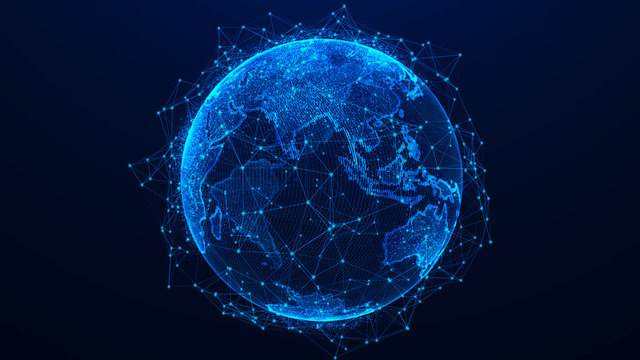
\includegraphics[width=0.5\textwidth]{data.jpg}
    \caption{Globale Daten verknüpft mit dem Internet}
    \label{fig:data}
\end{figure}

\section{Welche Daten werden geschützt?}

Die Arten von Daten, die durch die DSGVO geschützt sind, sind personenbezogene Daten wie Namen, Adressen, Telefonnummern, E-Mail-Adressen, etc. Diese Daten sind geschützt, um die Privatsphäre und die Rechte der betroffenen Personen zu wahren. Beispiele für geschützte Daten sind Kundendaten, Mitarbeiterdaten und Lieferantendaten. Es ist wichtig, diese Datenethik zu beachten, um das Vertrauen der Kunden zu gewinnen und zu erhalten. Durch Maßnahmen wie Datenverschlüsselung und Datenintegrität können Risiken wie Ransomware und Datenmanipulation minimiert werden, was wiederum das Vertrauen der Kunden stärkt. \textit{"Daten sind durch die DSGVO geschützt" \Citep{data-wbs}}

\section{Wie und warum werden Daten verkauft?}

Daten werden verkauft, indem Datenhändler sie an andere Unternehmen weitergeben, die sie für kommerzielle Zwecke nutzen. Datenhändler verkaufen Informationen wie persönliche Daten, Kaufverhalten, Interessen und andere relevante Informationen an Unternehmen, die diese Daten für ihre Marketing- und Geschäftsstrategien verwenden. Die Legalität des Handels mit Daten variiert von Land zu Land und die Rechtslage ist nicht immer eindeutig. Wenn Datenhändler ihre Informationen aus öffentlich zugänglichen Quellen beziehen, bewegen sie sich in der Regel auf der legalen Seite. \textit{"Neben den ethischen und juristischen Fragen, die der Datenhandel aufwirft, ist es das Ausmaß an Datenschutzverletzungen, das Anlass zur Sorge gibt. Datenhändler häufen vertrauliche Daten an, die in den falschen Händen für die Betroffenen schwerwiegende Konsequenzen haben können" \Citep{data-kaspersky}}